\documentclass[14pt]{extbook}
\usepackage{multicol, enumerate, enumitem, hyperref, color, soul, setspace, parskip, fancyhdr} %General Packages
\usepackage{amssymb, amsthm, amsmath, latexsym, units, mathtools} %Math Packages
\everymath{\displaystyle} %All math in Display Style
% Packages with additional options
\usepackage[headsep=0.5cm,headheight=12pt, left=1 in,right= 1 in,top= 1 in,bottom= 1 in]{geometry}
\usepackage[usenames,dvipsnames]{xcolor}
\usepackage{dashrule}  % Package to use the command below to create lines between items
\newcommand{\litem}[1]{\item#1\hspace*{-1cm}\rule{\textwidth}{0.4pt}}
\pagestyle{fancy}
\lhead{Makeup Progress Quiz 2}
\chead{}
\rhead{Version B}
\lfoot{2790-1423}
\cfoot{}
\rfoot{Summer C 2021}
\begin{document}

\begin{enumerate}
\litem{
For the graph below, find the value(s) $a$ that makes the statement true: $ \displaystyle \lim_{x \rightarrow a} f(x) = 0$.
\begin{center}
    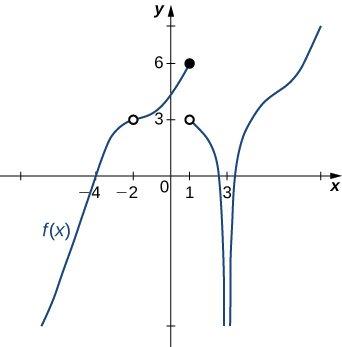
\includegraphics[width=0.5\textwidth]{../Figures/evaluateLimitGraphicallyB.png}
\end{center}
\begin{enumerate}[label=\Alph*.]
\item \( 3 \)
\item \( -4 \)
\item \( 0 \)
\item \( \text{Multiple } a \text{ make the statement true}. \)
\item \( \text{No } a \text{ make the statement true}. \)

\end{enumerate} }
\litem{
Evaluate the one-sided limit of the function $f(x)$ below, if possible.\[ \lim_{x \rightarrow 7^+} \frac{1}{(x-7)^6}+1 \]\begin{enumerate}[label=\Alph*.]
\item \( -\infty \)
\item \( \infty \)
\item \( f(7) \)
\item \( \text{The limit does not exist} \)
\item \( \text{None of the above} \)

\end{enumerate} }
\litem{
For the graph below, find the value(s) $a$ that makes the statement true: $ \displaystyle \lim_{x \rightarrow a} f(x) = -\infty$.
\begin{center}
    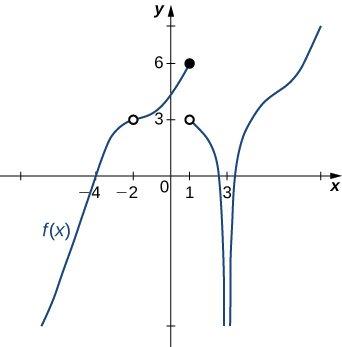
\includegraphics[width=0.5\textwidth]{../Figures/evaluateLimitGraphicallyCopyB.png}
\end{center}
\begin{enumerate}[label=\Alph*.]
\item \( 3 \)
\item \( -2 \)
\item \( -\infty \)
\item \( \text{Multiple } a \text{ make the statement true}. \)
\item \( \text{No } a \text{ make the statement true}. \)

\end{enumerate} }
\litem{
Evaluate the limit below, if possible.\[ \lim_{x \rightarrow 7} \frac{\sqrt{9x - 27} - 6}{2x - 14} \]\begin{enumerate}[label=\Alph*.]
\item \( \infty \)
\item \( 1.500 \)
\item \( 0.042 \)
\item \( 0.083 \)
\item \( \text{None of the above} \)

\end{enumerate} }
\litem{
Evaluate the limit below, if possible.\[ \lim_{x \rightarrow 4} \frac{\sqrt{8x - 16} - 4}{6x - 24} \]\begin{enumerate}[label=\Alph*.]
\item \( 0.167 \)
\item \( \infty \)
\item \( 0.021 \)
\item \( 0.125 \)
\item \( \text{None of the above} \)

\end{enumerate} }
\litem{
Evaluate the one-sided limit of the function $f(x)$ below, if possible.\[ \lim_{x \rightarrow -9^-} \frac{-4}{(x-9)^6}+5 \]\begin{enumerate}[label=\Alph*.]
\item \( \infty \)
\item \( -\infty \)
\item \( f(-9) \)
\item \( \text{The limit does not exist} \)
\item \( \text{None of the above} \)

\end{enumerate} }
\litem{
To estimate the one-sided limit of the function below as $x$ approaches 10 from the right, which of the following sets of numbers should you use?\[ \frac{\frac{10}{x} - 1}{x - 10} \]\begin{enumerate}[label=\Alph*.]
\item \( \{ 10.0000, 9.9000, 9.9900, 9.9990 \} \)
\item \( \{ 10.1000, 10.0100, 10.0010, 10.0001 \} \)
\item \( \{ 9.9000, 9.9900, 9.9990, 9.9999 \} \)
\item \( \{ 10.0000, 10.1000, 10.0100, 10.0010 \} \)
\item \( \{ 9.9000, 9.9900, 10.0100, 10.1000 \} \)

\end{enumerate} }
\litem{
To estimate the one-sided limit of the function below as $x$ approaches 7 from the left, which of the following sets of numbers should you use?\[ \frac{\frac{7}{x} - 1}{x - 7} \]\begin{enumerate}[label=\Alph*.]
\item \( \{ 6.9000, 6.9900, 7.0100, 7.1000 \} \)
\item \( \{ 6.9000, 6.9900, 6.9990, 6.9999 \} \)
\item \( \{ 7.0000, 6.9000, 6.9900, 6.9990 \} \)
\item \( \{ 7.0000, 7.1000, 7.0100, 7.0010 \} \)
\item \( \{ 7.1000, 7.0100, 7.0010, 7.0001 \} \)

\end{enumerate} }
\litem{
Based on the information below, which of the following statements is always true?
\begin{center}
    \textit{ $f(x)$ approaches $5.448$ as $x$ approaches $7$. }
\end{center}
\begin{enumerate}[label=\Alph*.]
\item \( f(x) \text{ is close to or exactly } 7 \text{ when } x \text{ is close to } 5.448 \)
\item \( f(x) = 7 \text{ when } x \text{ is close to } 5.448 \)
\item \( f(x) = 5.448 \text{ when } x \text{ is close to } 7 \)
\item \( f(x) \text{ is close to or exactly } 5.448 \text{ when } x \text{ is close to } 7 \)
\item \( \text{None of the above are always true.} \)

\end{enumerate} }
\litem{
Based on the information below, which of the following statements is always true?
\begin{center}
    \textit{ As $x$ approaches $2$, $f(x)$ approaches $5.809$. }
\end{center}
\begin{enumerate}[label=\Alph*.]
\item \( f(2) \text{ is close to or exactly } 5 \)
\item \( f(5) = 2 \)
\item \( f(2) = 5 \)
\item \( f(5) \text{ is close to or exactly } 2 \)
\item \( \text{None of the above are always true.} \)

\end{enumerate} }
\end{enumerate}

\end{document}